\documentclass{article}
%\usepackage[showframe,headsep=1cm,headheight=2cm]{geometry}. 
%\usepackage{fullpage} % Include this if you want to cram lots of things on a page
 
\usepackage{amsmath} % these are standard macro packages of the American Mathematical Society
\usepackage{amssymb}
\usepackage{hyperref}
\usepackage{cite}
%\usepackage{stmaryrd}


\usepackage{epsfig} % if you want figures
\usepackage{subfigure}
\usepackage{wrapfig}


\usepackage{fancyhdr} % These 4 lines are needed to set up the running  header
\fancyhead[LE,RO]{Sensor Overlays for Google map}
\fancyhead[RE,LO]{\thepage}
\pagestyle{fancy}





\newcommand{\matlab}[1]
{\centerline{\parbox{.9\textwidth}{\noindent\textsc{\bf MATLAB:} #1}}}

\newcommand{\code}[1]{\texttt{#1}}

\newcommand {\x}{\V{x}}
\newcommand {\y}{\V{y}}
\newcommand {\V}[1]{\mbox{\boldmath$#1$}}

\begin{document}
\title{Sensor Overlays for Google Map}
\author{Xiuhan Hu (xh2234@columbia.edu)}
\maketitle
\mbox{}
\section{Introduction}

The Web of Tings (WoT) allow real-world objects to be part of the World Wide Web, and users can view or manipulate things easily via the Internet. To visualize sensors on a map is essential to achieve WoT, since we often need to know the remote environment in a panoramic view before we change specific things. 

The goal of the project, Sensor Overlay for Google Maps, is to find a way to display information from the sensors as an overlay on Google Maps. The map view should be updated in real-time and work without user intervention most of time. There are innumerable kinds of sensors in real world, so the user should be able to customize the appearance according to the state of sensors. Another problem is that if there are too many sensors in a narrow space, the map view will be too crowded to be readable, unless we can cluster the sensors in a reasonable way. Existing solutions do not provide a realtime updating interface with automatically clustering function \cite{nath2006sensormap}.

In section 2, the structure of overall system and the user interface facilities are described briefly, which explains the real-time updating feature of the map. Section 3 shows how a sensor descriptor is defined and how sensors can be rendered with different shapes, icons and colors. The solution for sensor clustering problem is covered in Section 4. Concluding remarks are given in Section 5 . 

\section{Overall Structure}

The map interface need to provide real-time updated value of sensors. It should be able to communicate with sensors in certain way. However, it is costly for the interface to talk to individual sensors directly. So a sensor proxy service is created that the interface can establish a WebSocket connection to [Fig \ref{fig:overall:a}]. The service provides basic information about a sensor as a sensor descriptor and it also provides an API for the interface to subscribe to the sensor. The following shows how the system will response to a viewer [Fig \ref{fig:overall:b}]. 1) The map interface request all available sensor descriptors from sensor proxy service. 2) The sensor proxy service will consult sensor config service, and the config service will collect information from sensors to build sensor descriptors, combine descriptors with their geometry models and return those descriptors to the map interface via sensor proxy service. 3) Then for each sensor, the map interface will subscribe to it through sensor proxy service. 4) The sensor proxy will keep querying the latest updates from subscribed sensors, and notify the interface of the updated values at intervals.

\begin{figure}[htbp]
\centering
\subfigure[Components]{\label{fig:overall:a}
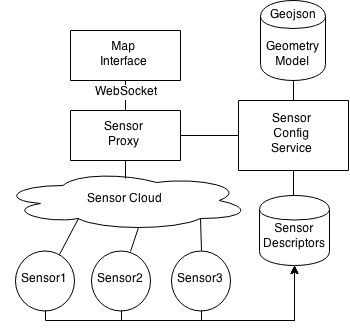
\includegraphics[width=0.4\columnwidth]{overallstructure.png}
}
\subfigure[Sequence Diagram]{\label{fig:overall:b}
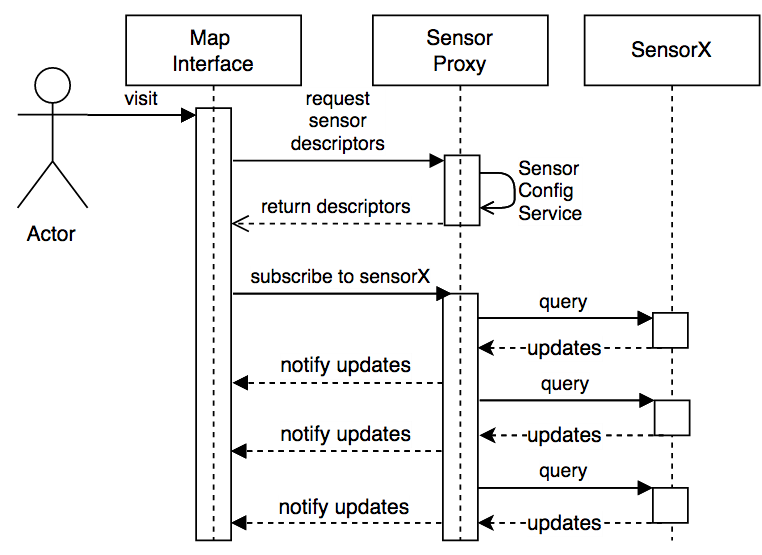
\includegraphics[width=0.4\columnwidth]{sequencedig.png}
}
\caption{Overall Structure}\label{fig:overall}
\end{figure}

Now the map interface can get the updated values of sensors.

\section{Sensor Descriptor And Rendering}

A sensor is rendered as a marker on the map interface, and its location or geometry is provided by its corresponding sensor descriptor. To generally describe all kinds of sensors, sensor descriptors should be well-defined in an abstract way. 

We classify sensors into two general types [Fig \ref{fig:sensortype}]: environmental sensors and structural sensors. 

\begin{figure}[htbp]
\centering
\subfigure[Environmental]{\label{fig:sensortype:a}
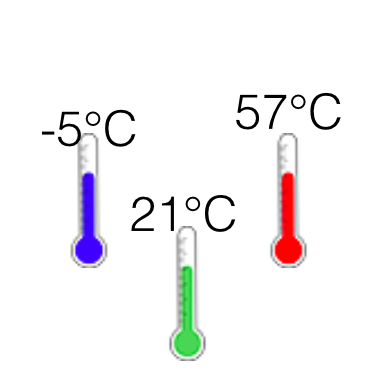
\includegraphics[width=0.3\columnwidth]{env.png}
}
\subfigure[Structural]{\label{fig:sensortype:b}
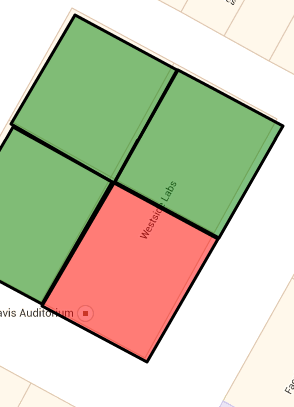
\includegraphics[width=0.2\columnwidth]{struct.png}
}
\caption{Two types of sensors}\label{fig:sensortype}
\end{figure}

An environment sensor provides information about the environment (ambient temperature, humidity, light intensity) in form of a number at certain location. A structural sensor reports on the state of a particular physical object (door open/close, lights on/off) in a certain shape recorded in our geometry model database.

We also want the appearance of the sensor marker to reflect the sensor's value. For example, the icon of thermometer marker will change from green to blue when it is getting too cold.

Taking account the above discussion, we borrow ideas from web design to build a sensor descriptor.

\begin{table}[h]
\begin{center}
\begin{tabular}{c|cc}
 & Web & Sensor Descriptor \\ \hline
Look \& Formatting & CSS & SensorStyle \\ 
Structure \& Content & HTML & SensorGeometry \& SensorData\\
Dynamic Altering & Javascript & SensorScript \\
\end{tabular}
\end{center}
\caption{Sensor Descriptor components and their counterparts in web design}\label{table:sensordes}
\end{table}


\begin{figure}[htb]
\centering
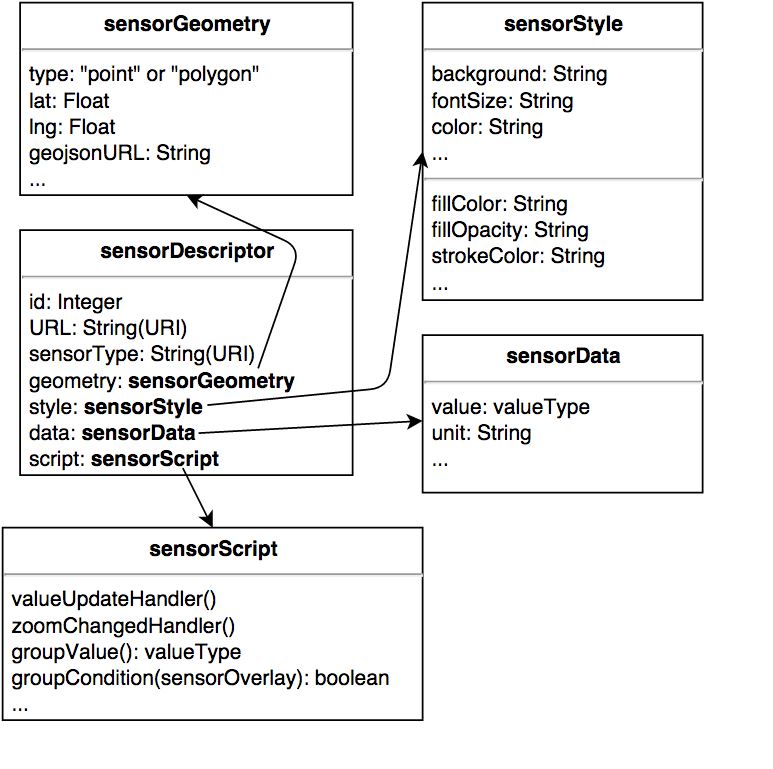
\includegraphics[width=0.8\columnwidth]{SensorDescriptor.png}
\caption{Sensor Descriptor Class Diagram}\label{fig:sensordes}
\end{figure}

As shown in Figure \ref{fig:sensordes}, the \textit{SensorStyle} part of \textit{SensorDescriptor} describes how the sensor marker looks like on the map interface. The \textit{SensorGeometry} part describes the location and shape of the sensor, which can cover all kinds of geometry information need for both types of sensors. The \textit{SensorData} gives the value and other relevant data for the sensor. The \textit{SensorScript} specifies how a sensor marker will change according to a recent event. The loose coupled structure of a sensor descriptor enable us to reuse certain parts of it conviniently.

When the interface need to show a sensor on the map, it will initialize an instance of \textit{SensorOverlay} from the given \textit{SensorDescriptor}, which copies the information from the \textit{SensorDescriptor} object to the new \textit{SensorOverlay} object. Then that \textit{SensorOverlay} object will draw itself on the map and register several event handler functions according to \textit{SensorScript}. 

To explain it more specifically, the following Figure \ref{fig:sensorupdate} shows how valueUpdateHandler() will be invoked.

\begin{figure}[htb]
\centering
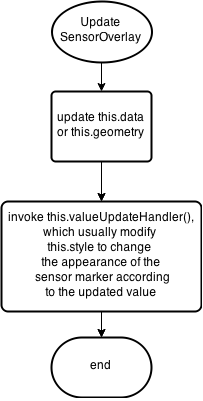
\includegraphics[width=0.2\columnwidth]{update.png}
\caption{Sensor Update}\label{fig:sensorupdate}
\end{figure}

The map interface will draw the sensor marker again after updating. The user will know there is a significant event (eg. temperature out of range) if a sensor marker changes its appearance obviously.



\section{Sensor Clustering}

If we have too many sensors to display in a small map area, the map will be unreadable for our users. Thus, automatically clustering sensors in that case is desirable for our map interface\cite{coleman1998clustering}. In \textit{SensorScript}, we define groupCondition() function to determine whether a sensor should be clustered with another sensor. groupCondition() function accept another \textit{SensorOverlay} object as input and return true if that sensor is getting too close to this sensor. 

When the zoom level of the map is changed by user, we first randomly choose several delegate sensors. Then we check other sensors by groupCondition() function to cluster them with right delegate sensors, and hide them from the map view. After we get clusters of sensors, we can calculate the integrated value of a cluster by a predefined function groupValue(). Then all \textit{SensorOverlay}'s zoomChangedHandler() function fires to finish the clustering process.

\begin{wrapfigure}{r}{0.35 \textwidth}
	\begin{flushright}
		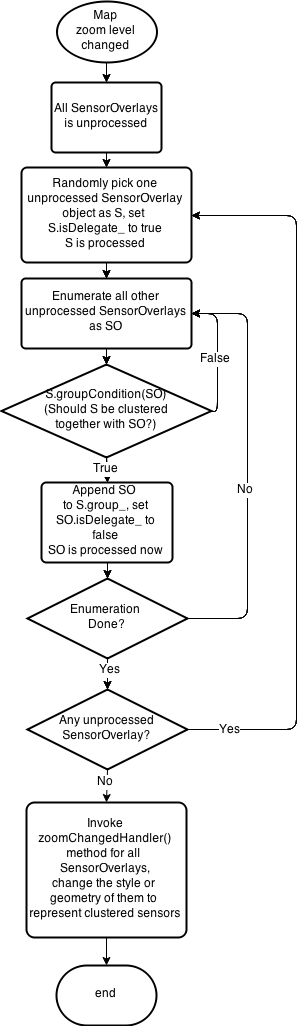
\includegraphics[width=0.3\textwidth]{clustering.png}
	\end{flushright}
	\caption{Zoom level changed}
	\label{fig:clustering}
\end{wrapfigure}


Figure \ref{fig:clustering} shows how the map will response to a zoom level change event. For environmental sensors, we probably want to know the average value of a cluster of sensors, so the groupValue() for them should be an arithmetic average function. For structural sensors, for example the door open/closed sensors, we need to warn the user if any sensor is in abnormal state, so the groupValue() for them should be a logic OR operation. The groupValue() can be generally considered a reduce function for a set of sensor values.

Figure \ref{fig:e} shows how thermometers are clustered when zoom level is changed.

It is more complicated to visualize clustered structural sensors, we need to specify how we want to change the shape of delegate sensor map. In many cases, we can draw a convex hull covering all clustered sensors [Fig \ref{fig:s}].




\section{Conclusion}

A sensor simulator instead of a real world sensor cloud is set for testing our map interface. The interface works well with current test setting and can provide clear and meaningful information for users. Reviewers can understand the interface with few explanation and no difficulties.

Through implementing the map interface, we have recognized that visualization should be semantic and information conveyed to user should be restrained. To improve our map, we can define more event handlers for sensor markers for a more versatile application.

In conclusion, the interface we designed is a solid step toward a general-purpose sensor visualization on a map view, which provide adequate information and a lighter burden of recognition for users.

\newpage

\begin{figure}[htb]
\centering
\subfigure[zoom=20]{\label{fig:e:a}
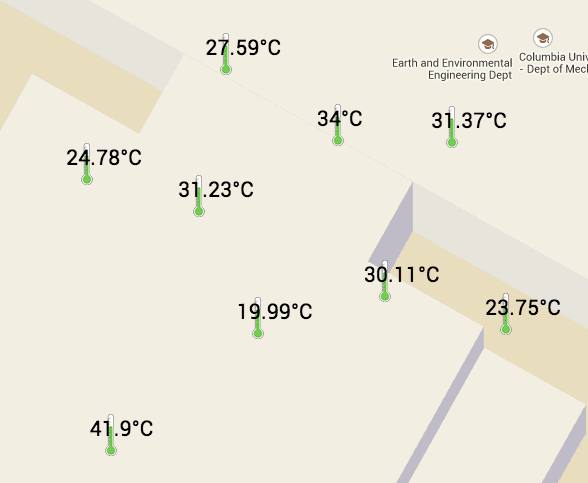
\includegraphics[width=0.3\textwidth]{e0.png}
}
\subfigure[zoom=19]{\label{fig:e:b}
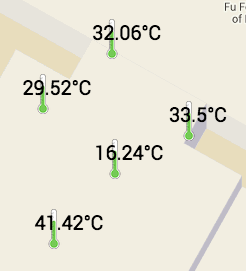
\includegraphics[width=0.2\textwidth]{e1.png}
}
\subfigure[zoom=18]{\label{fig:e:c}
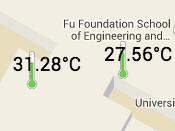
\includegraphics[width=0.15\textwidth]{e2.png}
}
\caption{Enviromental sensor clustering}\label{fig:e}
\end{figure}

\begin{figure}[htb]
\centering
\subfigure[zoom=20]{\label{fig:s:a}
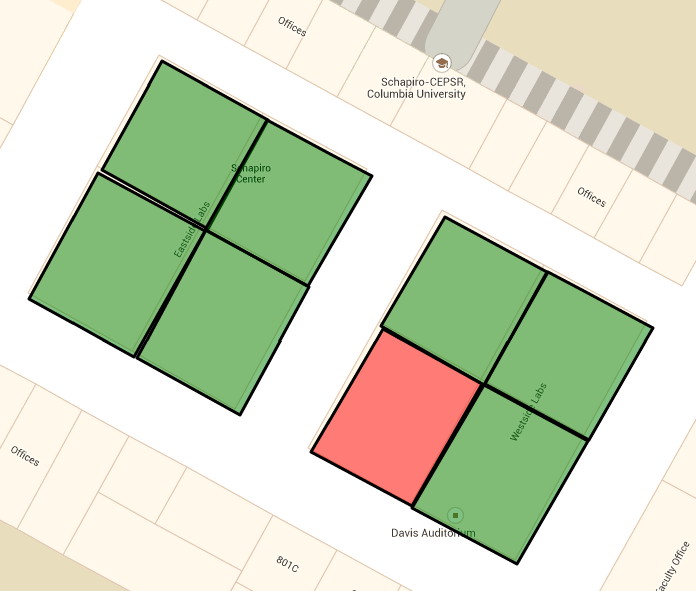
\includegraphics[width=0.3\textwidth]{s0.png}
}
\subfigure[zoom=19]{\label{fig:s:b}
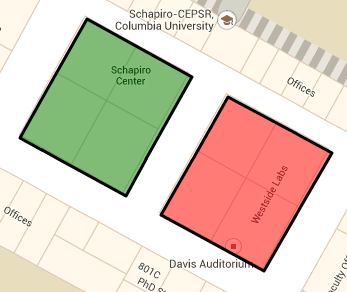
\includegraphics[width=0.2\textwidth]{s1.png}
}
\subfigure[zoom=18]{\label{fig:s:c}
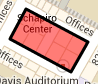
\includegraphics[width=0.15\textwidth]{s2.png}
}
\caption{Structural sensor clustering}\label{fig:s}
\end{figure}


\bibliography{report}{}
\bibliographystyle{plain}

\end{document}


